\documentclass[../../main.tex]{subfiles}

% 

\begin{document}
\chapter{Systémy pre ukladanie a spracovanie signálu z detektorov}

\section{Elektronika a príklady jednoduchých detekčných systémov}
Elektronika je kľúčovou súčasťou všetkých moderných detekčných systémov. Účelom front-end elektroniky a systémov na spracovanie signálu je
\begin{itemize}
\item Nadobudnutie (získání) elektrického signálu zo snímača. Typicky sa jedná o krátky elektricky impulz.
\item Prispôsobenie časovej odpovedi systému na optimalizáciu minimálneho detekčného systému, energetického merania, času príchodu, necitlivosti senzora na tvarovanie signálu alebo kombinácia týchto efektov.
\item Digitalizácia signálu a jeho následné uloženie na neskoršiu analýzu
\end{itemize}
Aj keď sú konfigurácie detektorov pomerne dosť zložité, vyžaduje sa použitie len niekoľkých základných princípov získavania signálu. Existujú niektoré spoločné základné prvky vyčítaciech systémov. Front-end obsahuje predzosilňovač, tvarovač pulzu, vyrovnávaciu pamäť a digitalizér , ktorý konvertuje bežný analógový vstup na digitálny výstup. V dnešných, vysoko energických fyzikálnych systémoch prakticky všetky detektory vyžadujú konverziu primárnej detekcie na elektrické signály.

Existujú dva základné typy detektorov, ktoré môžme rozdeliť podľa produkcie signálu
\begin{itemize}
\item Priama produkcia signálu: Pri priamom zisťovaní sa absorbovaná energia premieňa priamo na náboj, tj. elektrón-ión, elektrón-diera pár.
Napríklad v driftových komorách, mnoho-káblových proporcionálnych komorách (MWPC), ionizačných komorách (kalorimetre), polovodičových detektoroch (stripové a pixelové)
\item Nepriama produkcia: Nepriame detektory sú primárne scintilačné detektory, kde sa scintilačné svetlo mení na elektrický signál rôznymi technikami. Napríklad vo fotonásobičoch, polovodičových fotodiódach, lavínových fotodiódach, polovodičových fotonásobičoch.
\end{itemize}

\begin{figure}[!h]
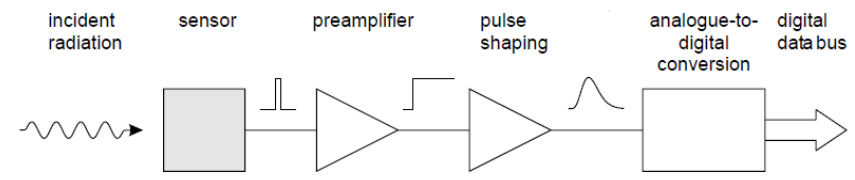
\includegraphics[width=1.0\textwidth]{emsf-10-schema.png}
\centering
\caption{Schéme priamej detekcie signálu.}
\label{em10:fig:priamaschema}
\end{figure}

Na obrázku (\ref{em10:fig:priamaschema}) môžme vidieť príklad schémy priamej detekcie signálu. Senzor konvertuje energiu uloženú nabitou časticou (alebo fotónovou) na elektrický signál. Vytvorený signálny náboj môže byť dosť malý, preto je potrebné signál senzora zosilniť. Veľkosť signálu senzora je predmetom štatistických výkyvov a elektronický šum ďalej rozmazáva signál, predzosilňovač musí byť starostlivo navrhnutý tak, aby sa minimalizoval elektronický šum. Dôležitým parametrom je kapacita senzora a kapacita zosilňovača pretože pomer signál-šum narastá s narastajúcou kapacitou. 

Príspevok elektronického šumu závisí kriticky aj od ďalšej fázy, tvarovača pulzu, ktorý určuje šírku pulzu systému a tým aj celkový príspevok elektronického šumu. Tvarovač tiež obmedzuje trvanie impulzu, ktorý nastavuje maximálnu možnú frekvenciu signálu. Výstup tvarovača pulzu smeruje do analog-digital konvertora (ADC), ktorý konvertuje veľkosť analógového signálu na bitový vzorku vhodnú pre následné digitálne ukladanie a spracovanie.

\begin{figure}[!h]
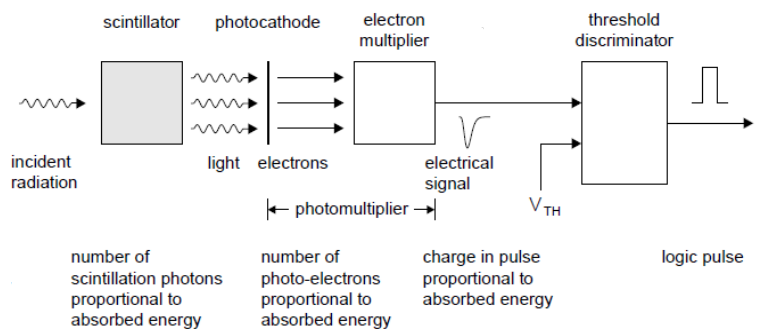
\includegraphics[width=1.0\textwidth]{emsf-10-schema1.png}
\centering
\caption{Schéme nepriamej detekcie signálu.}
\label{em10:fig:nepriamaschema}
\end{figure}

Na obrázku (\ref{em10:fig:nepriamaschema}) môžme pre zmenu vidieť príklad schémy nepriamej detekcie signálu. Scintilačný detektor využíva nepriamu detekciu, pričom najskôr sa absorbovaná energia premení na viditeľné svetlo. Nastáva zvýšenie amplitúdy pomocou elektrónového násobiča. Signál na výstupu fotonásobiča (PMT) je prúdový impulz, integrovaný v priebehu času. Tento impulz obsahuje signálny náboj, ktorý je úmerný absorbovanej energii. PMT výstupný impulz je privádzaný priamo do prahového diskriminátora, ktorý sa zapne, keď signál prekročí vopred určenú prahovú hodnotu ($V_{TH}$). Elektrónový násobič môže poskytnúť dostatočný zisk, takže nie je potrebný žiadny predzosilňovač.

\section{Signálna integrácia}
Signál zo senzoru je zvyčajne krátky prúdový pulz, $i_s(t)$. Avšak, fyzikálna veličina, ktorá nás zaujíma je častokrát depozitovaná energia v detektore. Nato aby sme ju získali musíme vyintegrovať cez všetky prúdové pulzy
$$ E \sim Q_s = \int i_s(t)dt.$$
Táto integrácia môže byť vykonaná v ľubovoľnej fáze lineárneho systému, takže je možné
\begin{itemize}
\item integrovať na senzorovej kapacite
\item použitie integrujúceho predzosilňovača - nábojovo-závislý predzosilňovač
\item rýchlo odobrať a digitalizovať aktuálny impulz a sčítať numericky
\end{itemize}

Keď sa mobilné nosiče nábojov pohybujú smerom k elektródam, menia indukovaný náboj na senzorových elektródach, ktoré tvoria kondenzátor $C_d$. Ak má zosilňovač veľmi malý vstupný odpor $R_i$, potom časová konštanta, $T = R_i(C_d+C_i)$, na vybitie snímača je malá, a zosilňovač bude cítiť signálny prúd. $C_i$ je dynamická vstupná kapacita, viď (\ref{em10:fig:inter}). Ak je vstupná časová konštanta veľká v porovnaní s trvaním prúdového pulzu potom bude prúdový pulz integrovaný na senzorovej kapacite a výsledné napätie na vstupe zosilňovača bude
$$ V_i = \frac{Q_s}{C_d + C_i}. $$ Takže vidíme, že veľkosť signálu závisí od kapacity senzora. V systéme s rôznymi kapacitami senzorov by sme sa museli vysporiadať s ďalšími kalibráciami. 

\begin{figure}[!h]
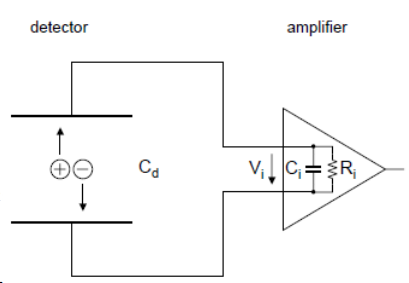
\includegraphics[width=0.6\textwidth]{emsf-10-inter.png}
\centering
\caption{Schéma vyintegrovania signálu.}
\label{em10:fig:inter}
\end{figure}

\section{Elektronický šum}
Uvažujme prúd prúdiaci cez vzorku, ktorá je ohraničenú dvoma elektródami. tj. pohybujúcich sa $n$ elektrónov s rýchlosťou $v$. Indukovaný prúd závisí na medzere $I$ medzi elektródami ako 
$$ i = \frac{nev}{I}.$$
Fluktuácia tohto prúdu je daná celkovým diferenciálom
$$ \langle di \rangle^2 = \bigg( \frac{ne}{I} \langle dv \rangle  \bigg)^2 + \bigg( \frac{ve}{I} \langle dn \rangle  \bigg)^2,$$
kde môžme sčítať tieto členy, keďže sú nekorelované. Z tohto vidíme, že dva mechanizmy prispievajú k celkovej fluktuácii šumu, rýchlosť a počet elektrónov. Fluktuácie v rýchlosti pochádzajú z termálneho pohybu. Zdrojom fluktuácii v počte nosičov je zachytávanie nosičov, pretože nedostatky v kryštálovej mriežke alebo nečistoty v plynoch môžu zachytávať nosiče nábojov a uvoľňovať ich po charakteristickej dobe.

\section{Tvarovanie pulzu}
Impulzové tvarovanie má dva protichodné efekty. Prvým je obmedzenie šírky pulzu tak, aby zodpovedala času merania. Príliš veľká šírka pulzu zvýši šum bez zvyšovania signálu. Zvyčajne impulzový tvarovač transformuje úzky senzorový impulz do širšieho impulzu s postupne zaokrúhleným maximom v čase vrcholu $T_P$, viď obrázok (\ref{em10:fig:time}).

\begin{figure}[!h]
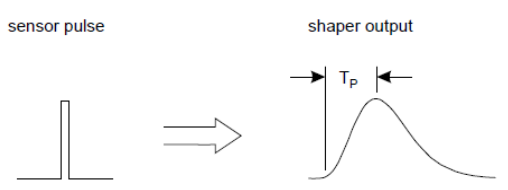
\includegraphics[width=0.6\textwidth]{emsf-10-time.png}
\centering
\caption{Zmena pulzu tvarovačom.}
\label{em10:fig:time}
\end{figure}

Druhým cieľom je obmedziť šírku impulzov tak, aby sa mohli merať po sebe idúce signálové impulzy bez prekrytia (bez pile-up), viď obrázok (\ref{em10:fig:pileup}). Pri navrhovaní tvarovača je potrebné vybalancovať tieto protichodné efekty. Optimálne tvarovanie závisí od aplikácie.

\begin{figure}[!h]
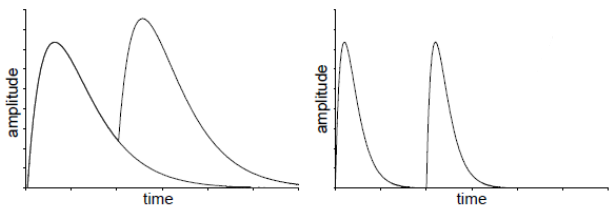
\includegraphics[width=0.6\textwidth]{emsf-10-pileup.png}
\centering
\caption{Znázornenie dvoch pulzov s rôznou oblasťou prekrytia.}
\label{em10:fig:pileup}
\end{figure} 

Signálny prúd zo snímača je integrovaný, aby vytvoril krokový impulz s dlhým rozpadom. Následný high-pass filter ("diferenciátor") obmedzuje šírku impulzu a low-pass filter ("integrátor") zvyšuje čas nábehu na vytvorenie impulzu s hladkým hrotom, viď obrázok (\ref{em10:fig:shaping}).

\begin{figure}[!h]
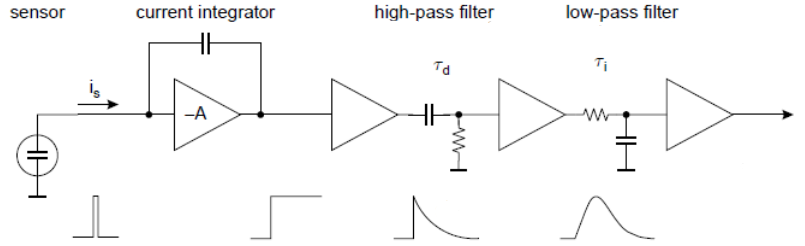
\includegraphics[width=0.9\textwidth]{emsf-10-shap.png}
\centering
\caption{Tvarovanie pulzu.}
\label{em10:fig:shaping}
\end{figure}

\section{Konverzia analógu na digitál}
Pre ukladanie údajov a následnú analýzu musí byť analógový signál na výstupnom formáte digitalizovaný. Dôležité parametre pre analógovo-digitálne meniče (ADC) použité v detekčných systémoch sú nasledovné:
\begin{itemize}
\item rozlíšenie: zrnitosť digitalizovaného výstupu
\item diferenciálna nelinearita: Ako jednotné sú prírastky digitalizácie?
\item integrálna nelinearita: Je digitálny výstup úmerný analógovému vstupu?
\item čas konverzie: Koľko času je potrebné na konverziu analógového signálu na digitálny výstup?
\item výpočetná rýchlosť: Ako rýchlo môže začať nová konverzia po dokončení predchádzajúcej konverzie bez zavedenia škodlivých artefaktov?
\item Stabilita: Menia sa parametre konverzie s časom?
\end{itemize}

Uvedieme nejaké metódy, ktorými sa prevádza analógový signál na digitálny: flash conversion ADC (najjednoduchšia),  successive-approximation ADC (najpoužívanejšia) alebo the Wilkinson ADC.

\section{Trigger system }
Trigger system experimentu je systém, ktorý v reálnom čase rozhoduje o tom, ktorú podmnožinu údajov z objemu detektora, detektor vyčíta a archivuje pre offline analýzu. Pekným a jednoduchým príkladom trigger-u: pri rozptylovom experimente budú zaznamenané len častice, ktoré sa rozptýlia pod uhlom $\theta$.

Pri nasledujúcom opise budeme vychádzať z Trigger systému, ktorý je používaný na experimente STAR. V jednoduchosti ide o to, že cely detektor môžme rozdeliť na pomalé detektory (jedná sa o tie hlavné detektory ako Time Projection Chamber alebo Heavy Flavor Tracker) a rýchle detektory (napríklad Beam-Beam counter, Zero Degree Calorimeter, Vertex Position Detector). Tieto pomalé detektory pod náporom obrovského množstva dát nedokážu analyzovať všetky udalosti, ktoré v detektore nastali. Preto je potrebné uľahčiť im prácu a to tak, že použijeme rýchle detektory, ktoré rozhodnú, či udalosť spadá do vopred zvolených kritérií. 

STAR Trigger systém je funkčne rozdelený na štyri rôzne úrovne - L0, L1, L2, L3. Interakcie, ktoré prechádzajú kritériami výberu v týchto po sebe nasledujúcich trigger úrovniach, sa posielajú do úložisk.

\subsubsection{Level 0:}
Tento level je najrýchlejší a analyzuje nespracované data a určuje, či sa požadovaný typ interakcie vyskytol v zrážke dvoch častíc. Údaje používané na tejto úrovni sú väčšinou z ZDC, BBC a VPD detektorov. Keď data spĺňajú podmienky tohto levelu tak pokročia do ďalšieho.

\subsubsection{Level 1, Level 2:}
Level 1 a 2 fungujú v časovom období niekoľkých milisekúnd, počas ktorých sa údaje analyzujú podrobnejšie, aby sa zistilo, či udalosť spĺňa viac jemnejšie požadované kritériá. Ak tomu tak nie je, proces digitalizácie sa preruší a detektory sa uvoľnia pre nový triggering.

\subsubsection{Level 3:}
Na tejto úrovni sa spraví konečné rozhodnutie. Ak údaje prechádzajú touto úrovňou, budú odoslané do úložiska. Tento level taktiež zahŕňa on-line zobrazenie, aby jednotlivé udalosti mohli byť vizuálne kontrolované v reálnom čase tj. že počas naberania dat si môže človek pozrieť aktuálny stav detektora.

\section{DAQ}
Systém DAQ (Data Acquisition) zhromažďuje dáta z rôznych častí detektora, konvertuje dáta do vhodného formátu a ukladá ich do trvalého ukladania. Požiadavky systému DAQ:
\begin{itemize}
\item poskytovanie online služieb (kontrola systému spustenia, monitorovanie toku dát, ovládanie detektorov atď.)
\item uchovanie záznamov o stave údajov a stave detektora
\item zabránenie poškodeniu dát
\item poskytnutie flexibility pri zaznamenávaní údajov v rôznych konfiguráciách (uvedenie do prevádzky, kalibrácia, fyzikálne spracovanie údajov)
\item minimalizácie doby nečinnosti
\item cenová dostupnosť
\end{itemize}

\begin{figure}[!h]
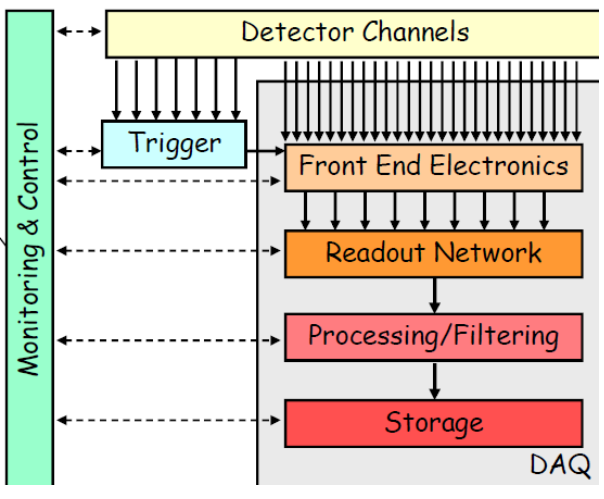
\includegraphics[width=0.5\textwidth]{emsf-10-DAQ.png}
\centering
\caption{Schéma DAQ systému.}
\label{em10:fig:daq}
\end{figure}

\begin{itemize}
\item DAQ systém zhromažďuje údaje vytvorené detektorom a uchováva ich (pre pozitívne trigger rozhodnutia).
\item Front-end elektronika prijíma signály od detektorov, triggerov, časovačov a produkuje dikitalizované informácie.
\item Readout network číta front-end data a formuje kompletné udalosti - event building.
\item Centrálne DAQ ukladá údaje o udalostiach, dokáže spracovať a filtrovať údaje.
\end{itemize}

\section{Mŕtva doba DAQ}
Mŕtva doba DAQ je zlomok času, ktorom experiment nemôže zaznamenať žiadne data. Medzi zdroje tohto mŕtveho času patri:
\begin{itemize}
\item mŕtva doba readout a trigger systému
\item Prevádzková mŕtve časy (napr. Začiatky/zastávky obdobia zberu dát)
\item T/DAQ down-time (napríklad zlyhanie počítača)
\item detektora down-time (napríklad po výpadku vysokého napätia)
\end{itemize}
Všimnite si, že logika mŕtveho času je potrebná, aby sa zabránilo spúšťaniu inej udalosti pred úplným odčítaním detektora. Systém T/DAQ musí byť navrhnutý tak, aby minimalizoval mŕtvy čas.

\section{Jednoduchý T/DAQ systém}
Uvažujme experiment určený na meranie času letu (TOF) častíc prechádzajúcich scintilačnými čítačmi. Tieto údaje budú vyčitané s elektronikou Time-to-Digital Converter (TDC), viď obrázok (\ref{em10:fig:tdaq}).

\begin{figure}[!h]
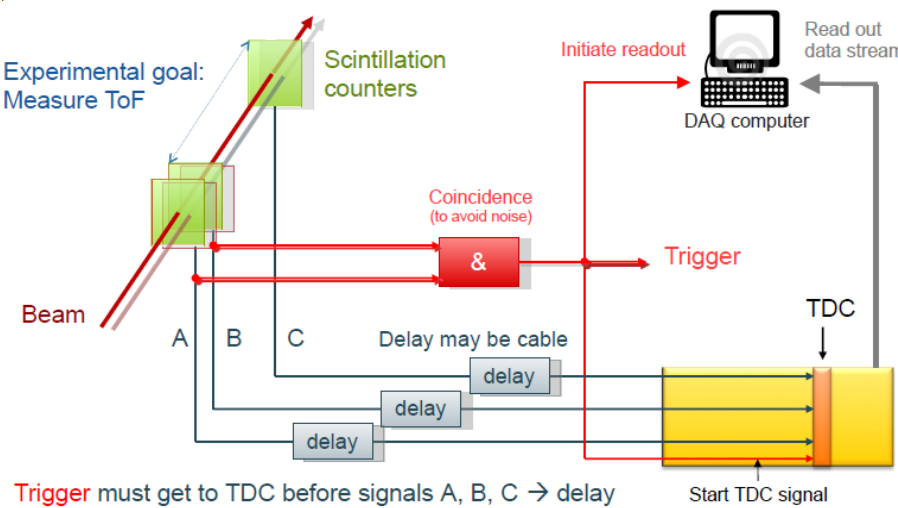
\includegraphics[width=0.87\textwidth]{emsf-10-TDAQ.png}
\centering
\caption{Schéma uvažovaného experimentu.}
\label{em10:fig:tdaq}
\end{figure}

Vzniknuté obmedzenia:
\begin{itemize}
\item trigger rozhodnutie musí byť veľmi rýchle aby sa spustilo TDC pred príchodom signálov A, B, C.
\item TDC vyčitanie do DAQ počítača je trochu pomalé.
\item významná mŕtva doba ak je trigger rozsah veľký: readout mŕtva doma = trigger rozsah $\times$ celkový readout time
\end{itemize}

\section{Multi-level trigger}
Často nemôžeme dosiahnuť požiadavky na vysokú efektivitu signálu a vysoké potlačenie pozadia s mimoriadne krátkym trigger oneskorením (zpožděním). Preto vzniká potreba zaviesť koncept multi-level trigger. Prvý trigger level má veľmi krátke oneskorenie, vysokú efektivitu signálu, ale skromné potlačenie pozadia. Niekedy sa nazýva pre-trigger. Následné trigger levely dosahujú vysoké potlačenie pozadia, s typicky vyšším oneskorením. Toto je vlastne to, čo sme už opisovali vyššie, keď sme opisovali trigger systém pre STAR experiment.

\section{Tok dát na ALICE}
Z hľadiska toku údajov je LHC veľmi komplexné potrubie toku údajov. Tieto údaje sa musia pohybovať nepretržite, pretože žiadna vyrovnávacia pamäť nie je dostatočne veľká na to, aby zvládla uchovať také množstvo údajov. Akékoľvek prerušenie toku dát vytvára vážne problémy. Údaje musia byť k dispozícii s veľmi krátkym oneskorením. Na obrázku (\ref{em10:fig:flow}) môžme vidieť čo schéma toku dát obsahuje.

\begin{figure}[!h]
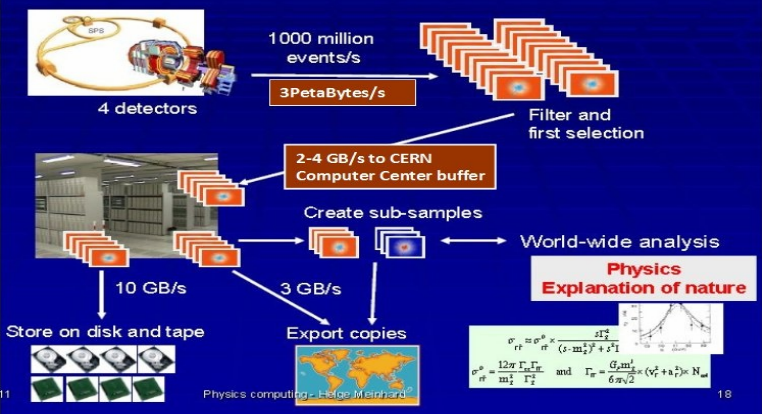
\includegraphics[width=0.8\textwidth]{emsf-10-flow.png}
\centering
\caption{Schéme toku dát na experimente ALICE.}
\label{em10:fig:flow}
\end{figure}

\section{ALICE trigger, DAQ a HLT}
Akronymy detektorov a systémov: 
\begin{itemize}
\item ECS: Experiment Control System
\item LTU: Local Trigger Unit - subdetektorové rozhranie
\item TRG: Trigger system
\item TTC: Trigger and Time control
\item CTP: Central Trigger Processor
\item DCS: Detector Control System
\item DAQ: Data Acquisition system
\item HLT: High Level Trigger
\item FERO: Front End ReadOut electronics - pripojený k detektoru dáva vstup DAQ
\item DDL: Detector Data Link - prepojenie medzi FERO and DAQ
\item LDC: Local Data Concentrator - vstupný bod pre DAQ, jeden alebo viac LDC sú priradené ku každému detektoru
\item GDC: Global Data Collector
\item Read-Out Receiver Card
\end{itemize}

\begin{figure}[h!]
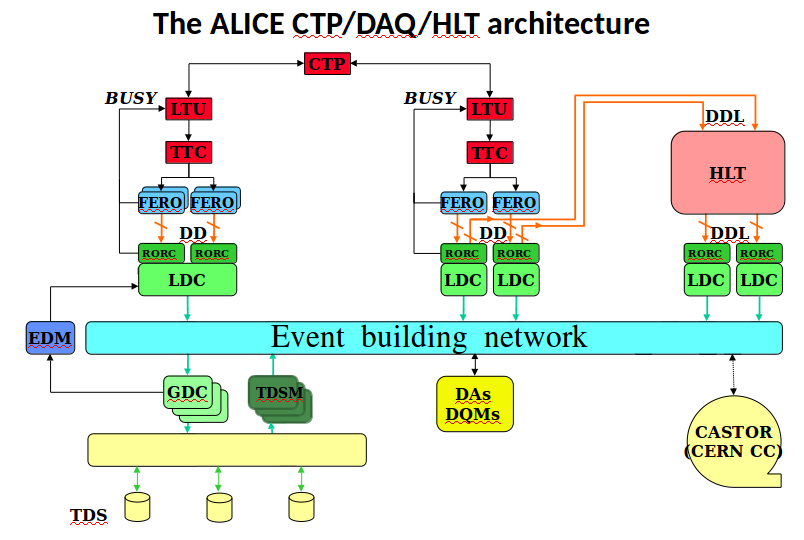
\includegraphics[width=1\textwidth]{emsf-10-architecture.png}
\centering
\caption{Architektúra experimentu ALICE.}
\label{em10:fig:architecture}
\end{figure}

\textbf{Jednotlivé systémy experimentu ALICE a proces tvorenia eventov:}
\begin{itemize}
\item Trigger - CTP $\rightarrow$ LTUs $\rightarrow$ TTC $\rightarrow$ FEROs
\item Výstup z detektora - FEROs $\rightarrow$ DDLs $\rightarrow$ RORCs - surové dáta z detektorov vstúpia do DAQ
\item Vstup do HLT - RORCs $\rightarrow$ Splitters $\rightarrow$ DDLs $\rightarrow$ HLT - vybrané časti údajov sú duplikované a odoslané do HLT
\item Spracovanie a výstup v HLT - HLT $\rightarrow$ DDLs $\rightarrow$ RORCs $\rightarrow$ LDCs - spracované údaje a rozhodnutia z HLT sa posielajú do DAQ.
\item Full-event - LDCs majú teraz full-event rozdelený do sub-eventov.
\item Sub-eventy môžu byť zlikvidované, nahradené alebo akceptované v súlade s rozhodnutím HLT.
\item Event building - LDCs $\rightarrow$ GDCs - akceptované sub-eventy sa posielajú na GDC, kde sú udalosti vytvorené/spojené.
\item Objektivizácia a nahrávanie - GDCs $\rightarrow$ TDS - udalosti sú objektivizované (vo formáte AliROOT) a zaznamenávané v TDS.
\item Migrácia - TDS $\rightarrow$ TDSM movers $\rightarrow$ Tier 0 - dátové bloky sa presunú z TDS do mriežky a zaregistrujú sa v Alien.
\item Online spracovanie - LDCs/GDCs $\rightarrow$ DAs/DQMs - časť údajov je spracovávaných online pomocou Detector Algorithms (DAs) a Data Quality Monitoring (DQM) modulov.
\end{itemize}

\section{Worldwide LHC Computing Grid (WLCG) - 20.6.2005}
Projekt Worldwide LHC Computing Grid (WLCG) je celosvetová spolupráca viac ako 170 výpočtových centier v 42 krajinách, ktoré spájajú národné a medzinárodné gridové infraštruktúry. Poslaním projektu WLCG je poskytnúť globálne výpočtové zdroje na ukladanie, distribúciu a analýzu približne 50 Petabajtov údajov očakávaných v roku 2018 generovaných Large Hadron Collider (LHC) v CERN. Rozloženie štruktúry WLCG môžme vidieť na obrázku (\ref{em10:fig:tier}).

\begin{itemize}
\item Tier 0: nahrávanie a archivovanie dát, prvotné rekonštrukcie dát, distribúcia dát - CERN + Wignerov inštitút
\item Tier 1: permanentné úložiska, centrálne riadená analýza, simulácie v niektorých prípadoch, opätovné spracovanie - 14 centier
\item Tier 2: simulácie, analýza koncového používateľa - viac ako 150 centier
\end{itemize}

\begin{figure}[h!]
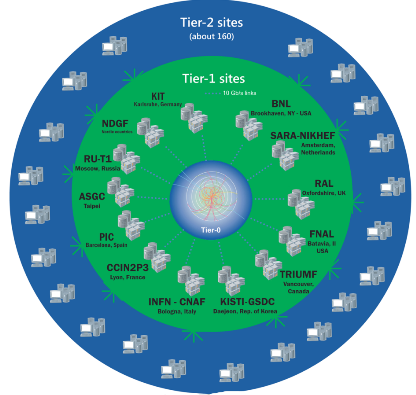
\includegraphics[width=0.9\textwidth]{emsf-10-tier.png}
\centering
\caption{Schéma rozloženia WLCG.}
\label{em10:fig:tier}
\end{figure}

Nato aby Wignerov inštitút patril do Tier 0 musí veľmi ale veľmi rýchlo dostávať dáta z CERN-u. Preto boli natiahnutá dva $100\,Gb/s$ káble medzi CERN-om a Wignerovým inštitútom (Maďarsko) na vytvorenie Tier 0 so sieťovým oneskorením (množstvo času, ktoré dáta potrebujú na presun z CERN-u do Wigner inštitútu) cca $25\,ms$.

\end{document}